% ==============================================================================
% TCC - Nome do Aluno
% Capítulo 2 - Revisão da Literatura
% ==============================================================================
\chapter{Revisão da Literatura}
\label{sec-literatura}

Neste capítulo é feita uma revisão dos principais conceitos utilizados neste
trabalho, além de apresentar fundamentos para uma compreensão mais profunda dos
mesmos.

\section{Redes Neurais Informadas pela Física}

Apresentadas em \cite{raissi-etal:19}, PINNs podem ser entendidas como uma forma
avançada de regularização, ou como um problema de otimização que transforma 
as condições de fronteira e iniciais em penalizações para a função custo. PINNs
são capazes de resolver problemas no seguinte formato: 

\begin{eqnarray}
    \mathcal{D}(u(\boldsymbol{x},t);\boldsymbol{\lambda}) &=& f(u,\boldsymbol{x},t), \quad \boldsymbol{x} \in \Omega, \, t \in I, \label{model-1-a}\\
    %
    \mathcal{B}(u(\boldsymbol{x},t)) &=& g(\boldsymbol{x},t), \quad \boldsymbol{x} \in \Gamma, \, t \in I, \label{model-1-b}\\
    %
    \mathcal{I}(u(\boldsymbol{x},t_0)) &=& q(\boldsymbol{x}), \quad \boldsymbol{x} \in \Omega, \label{model-1-c}
\end{eqnarray}

Em que $\Omega \subset \mathbb{R}^d$ é o domínio espacial limitado pela 
fronteira $\Gamma$; 
$d$ é a dimensão do domínio espacial; 
$T = [t_0, t_f]$ é o intervalo de tempo, sendo $t_0 < t_f$; 
$\boldsymbol{x} = (x_1, x_2, \dots, x_d)$ é um vetor de coordenadas espaciais; 
$t$ denota o tempo; 
$u = u(\boldsymbol{x}, t)$ denota a solução desconhecida do problema; 
$\boldsymbol{\lambda}$ é um vetor de parâmetros das equações; 
$\mathcal{D}$ é um operador diferencias associado às equações; 
$f$ é um termo fonte ou sorvedouro; 
$\mathcal{B}$ and $\mathcal{I}$ são operadores representando, respectivamente,
as condições de fronteira e iniciais; 
por fim, $g$ e $q$ são funções conhecidas que definem essas condições.

A equação \ref{eq:loss-fisica} define o termo da função de perda que engobla
todos as equações que compõem o modelo. Trata-se de um treinamento 
não-supervisionado que busca minimizar o residual definido.

\begin{equation}\label{eq:loss-fisica}
    \mathcal{L}_{\text{física}}(\boldsymbol{\theta}) 
    = \omega_{\text{domínio}} \mathcal{L}_{\mathcal{D}}(\boldsymbol{x},t,\boldsymbol{\theta}) 
    + \omega_{\text{fronteira}} \mathcal{L}_{\mathcal{B}}(\boldsymbol{x},t,\boldsymbol{\theta}) 
    + \omega_{\text{inicial}} \mathcal{L}_{\mathcal{I}}(\boldsymbol{x},t_0,\boldsymbol{\theta}) 
    %+ \omega_{data} J_{data}(\boldsymbol{x},t,\boldsymbol{\theta})
\end{equation}

Sendo $\omega_{\text{domínio}}$, $\omega_{\text{fronteira}}$ 
e $\omega_{\text{inicial}}$ pesos atribuídos a cada um dos residuais.
Caso haja dados disponíveis, é feito um treinamento supervisionado utilizando 
tais dados. A função de perda final da rede neural é então definida pela equação
\ref{eq:loss-total}.

\begin{eqnarray}\label{eq:loss-total} 
    \mathcal{L}_{\text{total}}(\boldsymbol{\theta}, \boldsymbol{\lambda}) 
    = \mathcal{L}_{\text{física}}(\boldsymbol{\theta}, \boldsymbol{\lambda}) 
    + \omega_{\text{dados}} \,\mathcal{L}_{\text{dados}}(\boldsymbol{\theta})
\end{eqnarray}

Aqui vale menciona que esta não é a única forma de distribuir os pesos da loss,
a implementação da biblioteca \textit{DeepXDE} \cite{lu-etal:21-deepxde}
permite atribuir pesos diferentes a cada condição inicial e de fronteira. 
Então o problema passa a ser encontrar os conjuntos $\boldsymbol{\theta}^*$ de 
parâmetros e viéses da rede, e o conjunto $\boldsymbol{\lambda}^*$ de parâmetros
das equações, que minimiza a função \ref{eq:loss-total}.

\begin{equation}\label{eq:otimizacao-parametros}
   (\boldsymbol{\theta}^*, \boldsymbol{\lambda}^*) 
   = \arg \min_{\boldsymbol{\theta}, \boldsymbol{\lambda}} \mathcal{L}_{\text{total}}(\boldsymbol{\theta}, \boldsymbol{\lambda}), 
\end{equation}

Existem muitos métodos de otimização para encontrar os argumentos 
da equação \ref{eq:otimizacao-parametros}. Pode-se citar o método de 
primeira ordem \textit{Adam} \cite{kingma-ba:14-adam} e o método quase-newtoniano
\textit{BFGS}, ou como comumente usado, a sua versão para ambientes de pouca
memória, o \textit{L-BFGS} \cite{liu-nocedal:89-lbfgs}.

A figura \ref{fig:pinn-representacao-grafica} mostra uma representação gráfica das 
PINNs.

\begin{figure}[htpb]
\centering
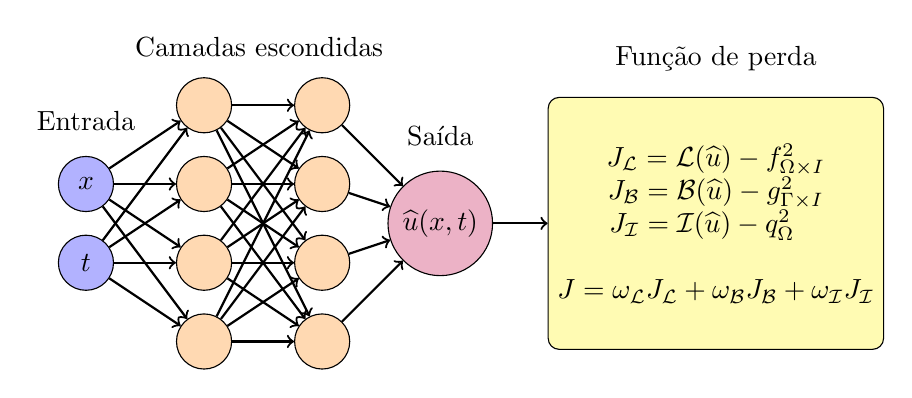
\begin{tikzpicture}[
    neuron/.style={circle, draw, minimum size=0.7cm},
    input/.style={neuron, fill=blue!30},
    hidden/.style={neuron, fill=orange!30},
    output/.style={neuron, fill=purple!30},
    physnode/.style={rectangle, draw, rounded corners, fill=orange!30, minimum width=1.5cm, minimum height=1.8cm},
    lossnode/.style={rectangle, draw, rounded corners, fill=yellow!30, minimum width=2cm, minimum height=3.2cm, align=center},
    every edge/.style={draw, ->, thick}
]

\node[input] (I-1) at (0, 2) {$x$};
\node[input] (I-2) at (0, 1) {$t$};

\node[hidden] (H1-1) at (1.5, 3) {};
\node[hidden] (H1-2) at (1.5, 2) {};
\node[hidden] (H1-3) at (1.5, 1) {};
\node[hidden] (H1-4) at (1.5, 0) {};

\node[hidden] (H2-1) at (3, 3) {};
\node[hidden] (H2-2) at (3, 2) {};
\node[hidden] (H2-3) at (3, 1) {};
\node[hidden] (H2-4) at (3, 0) {};

\node[output] (O-1) at (4.5, 1.5) {$\widehat{u}(x,t)$};

% Connections
\foreach \i in {1,2}
    \foreach \j in {1,...,4}
        \path (I-\i) edge (H1-\j);

\foreach \i in {1,...,4}
    \foreach \j in {1,...,4}
        \path (H1-\i) edge (H2-\j);

\foreach \j in {1,...,4}
    \path (H2-\j) edge (O-1);

\node[lossnode] (TotalLoss) at (8, 1.5) {
$J_{\mathcal{L}} = \lVert \mathcal{L}(\widehat{u}) - f \rVert^{2}_{\Omega \times I}$
\\
$J_{\mathcal{B}} = \lVert \mathcal{B}(\widehat{u}) - g \rVert^{2}_{\Gamma \times I}$
\\
$J_{\mathcal{I}} = \lVert \mathcal{I}(\widehat{u}) - q \rVert^{2}_{\Omega} \quad$
\\
\\
$J = \omega_{\mathcal{L}} J_{\mathcal{L}} + \omega_{\mathcal{B}} J_{\mathcal{B}} + \omega_{\mathcal{I}} J_{\mathcal{I}}$
};

\path (O-1) edge (TotalLoss);

% Labels
\node[above=0.2cm] at (I-1.north) {Entrada};
\node[above=0.2cm] at (2.2, 3.3) {Camadas escondidas};
\node[above=0.2cm] at (O-1.north) {Saída};
\node[above=0.2cm] at (TotalLoss.north) {Função de perda};

\end{tikzpicture}
\caption{Representação gráfica das PINNs. Fonte: elaborada pelos autores.}
\label{fig:pinn-representacao-grafica}
\end{figure}

A formulação acima vale tanto para problemas diretos, quanto para problemas 
inversos

\section{Modelos Compartimentais}

Baseados neste trabalho seminal,foram propostos outros modelos com mais mais 
compartimentos como o \textit{SEIRD} \cite{giles:77-sird} que inclui um 
compartimento para individuos que foram expostos a doença, mas 
ainda não manifestaram sintomas. 
Outro exemplo é o \textit{SIRV} \cite{schlickeiser-kroger:21-sirv} 
que inclui um compartimento para vacinados.

Em \cite{kendall:2023-modelos-epd-estocasticos}, é introduzido um modelo estocástico
baseado no trabalho já citado.

$R_0$ número básico

\begin{equation}
    R_0 = \frac{\beta}{\gamma}
\end{equation}

Apresentado no trabalho seminal de \cite{kermack-mcKendrick:1927}, o modelo 
\textit{SIR} é definido pelo conjunto de equações \ref{eq:SIR-1}, \ref{eq:SIR-2}
e \ref{eq:SIR-3}.

\begin{eqnarray}\label{eq:sir}
   \frac{dS(t)}{dt} &=& -\beta S(t) I(t),  \quad t > t_0, \label{eq:SIR-1}\\
   \frac{dI(t)}{dt} &=& \beta S(t) I(t) - \gamma I(t), \quad t > t_0, \label{eq:SIR-2}\\
   \frac{dR(t)}{dt} &=& \gamma I(t),  \quad t > t_0, \label{eq:SIR-3} \\
   S(t) + I(t) + R(t) &=& N,  \quad t > t_0, \label{eq:SIR-4}
\end{eqnarray}

O modelo pode ser entendido com um grafo\dots A figura \ref{fig:sir-grafo}
ilustra o modelo \textit{SIR}.

\begin{figure}
\centering
\begin{tikzpicture}[
    node distance=2.5cm,
    box/.style={rectangle, minimum width=2cm, minimum height=1.5cm, 
                draw=black, thick, align=center, rounded corners=5pt,
                font=\large\bfseries},
    arrow/.style={-Stealth, thick, line width=1.2pt},
    label/.style={midway, sloped, font=\small}
]

    % Define nodes
    \node[box, fill=blue!20] (S) {Susceptible \\ S(t)};
    \node[box, fill=red!20, right=of S] (I) {Infected \\ I(t)};
    \node[box, fill=green!20, right=of I] (R) {Recovered \\ R(t)};

    % Transitions
    \draw (S) edge[->] node[label,above] {$\beta$} (I);
    \draw (I) edge[->] node[label,above] {$\gamma$} (R);

\end{tikzpicture}
\caption{Grafo para o \textit{SIR}. Fonte: elaborada pelos autores.}
\label{fig:sir-grafo}
\end{figure}



\section{Problemas Inversos}

Problemas inversos são mal-postos\dots

Identificabilidade de um modelo\dots

\section{Aplicação de PINNs com Modelos Compartimentais}

\cite{}

Modelos de ordem facionária \cite{li-etal:25-ordem-fracionaria}

Sir reação-difusão \cite{bertaglia-etal:22-sir-reacao-difusao}

Um exemplo utilizando redes neurais recorrentes pode ser encontrado em \cite{rodriguez-etal:2022-einns}

No artigo original, são utilizados \textit{Multi-layer Perceptrons} (MLPs)
como arquitetura das redes, mas há propostas com utilizando outras arquiteturas.
Uma proposta utilizando redes neurais convolucionais pode ser encontrada em 
\cite{shi-etal:24-convnet}. Uma proposta utilizando PINNs combinado com 
métodos Bayesianos pode ser encontrada em \cite{yang:21-bpinns}, esta 
abordagem é particulamente interessante para problemas inversos, ao transformar
a estimativa dos parâmetros numa distribuição, no lugar de um valor fixo.
